\hypertarget{index_intro}{}\section{Introduction}\label{index_intro}
This code simulates the deformation of a viscoelastic medium in presence of a discrete fault under the anti-\/plane shear approximation. Under this assumption there is no displacement in the modeled plane $(v_{x}=v_{y}=0)$ and there is no spatial variation in the direction perpendicular to the modeled plane $(\partial z=0)$. If the case of a uniform shear modulus and shear viscosity, the problem is reduced to the Poisson equation where the right-\/hand side depends on the velocity values from the previous time step.

\begin{DoxyNote}{Note}
This code has been modified from deall.\-I\-I tutorial \href{https://www.dealii.org/8.2.0/doxygen/deal.II/step_31.html}{\tt step-\/31}.
\end{DoxyNote}
\hypertarget{index_equations}{}\subsection{Viscoelastic approximation}\label{index_equations}
We are interested in a system in which large deformations occur. In addition, we would like to take advantage of the methods that have already been studied. Therefore, we will try to adapt the equations that drive our problem so they resemble fluid flow equations, for which extensive research has been done regarding finite element methods and solving algorithms. For such purpose, we will start with the equation of conservation of momentum for an incompressible fluid\-: \[\partial_i{(\sigma_{ij})}=f_j\] where $i$ and $j$ run from 1 to 3 and designate spatial coordinate, $\sigma$ is the stress tensor and $f$ is the total external force, in this case, only the gravitational force $f_j=f^g_j=\rho g \left(1-\alpha T \right) \delta_{iy}$. The total stress can be separated in the deviatoric component $\tau_{ij}$ and pressure $P$\-: \[ \sigma_{ij} = \tau_{ij}-P \delta_{ij} \]

and the equation of conservation of motion will be\-: \[\partial_i \tau_{ij} - \partial_j P = \rho g \left( 1 - \alpha T \right) \delta_{jy} \]

Since we are going to use a semi-\/viscous approach we need a constitutive equation to relate the deviatoric stress and strain rate. For that, we will follow the approach from \cite{moresi_et_al_02} and \cite{moresi_et_al_03} and consider that the total deformation is acomodated by a linear combination of elastic and viscous deformation\-: \[ \dot \varepsilon = \dot \varepsilon^e + \dot \varepsilon^v = \frac{\check{\tau}}{2\mu} + \frac{\tau}{2\eta} \]

where $\dot\varepsilon$ is the strain rate, $\check{\tau}$ is the Jaumann corotatonal stress rate for an element of the continuum, $\mu$ is the shear modulus and $\eta$ is shear viscosity. The strain rate can be expressed in terms of the velocity of the continuum $u$\-: \[ \dot \varepsilon_{ij} = \frac{1}{2} \left( \partial_j v_i + \partial_i v_j \right) \]

The Jaumann derivative is an observer independent objective rate (see /cite harder\-\_\-91 for a discussion about the effect of using different objective derivatives on convection solutions). Jaumann stress can be expressed as\-: \[ \check{\tau} = \frac{D\tau}{Dt}+\tau\omega-\omega\tau\]

where $\omega$ is the material spin tensor, which can be expressed in terms of the velocity\-: \[\omega_{ij} = \frac{1}{2} \left( \partial_j v_i - \partial_i v_j \right) \]\hypertarget{index_num_approach}{}\subsection{Numerical approach}\label{index_num_approach}
To use a semi-\/viscous approach we need to manipulate the constitutive equation to write the deviatoric stress in terms of the strain rate (therefore in terms of derivatives of the velocity) and the substitute it in the momentum equation. This will give us an P\-D\-E of the velocities, which we will have to solve.\-To achieve this, the first step is to express the Jaumann stress rate as a first order difference form\-: \[\check{\tau} = \frac{\tau^t - \tau ^{t-1}}{\Delta t} + \tau^{t-1}\omega^{t-1} - \omega^{t-1}\tau^{t-1} \]

where the superscript $t$ indicates the current time step and $t-1$ the previous one, and $\Delta t$ is the time increment during the last step. The deviatoric stress tensor for the current time step can therefore be expressed in terms of the current strain rate and past deviatoric stress and material spin tensors\-: \[ \tau^t = 2 \eta_{ef} \dot\varepsilon^t + \eta_{ef} \left[\frac{1}{\mu\Delta t} \tau ^{t-1} + \frac {1}{\mu} \left( \omega^{t-1}\tau^{t-1} - \tau^{t-1}\omega^{t-1} \right) \right] \]

where $\eta_{ef}$ is an effective viscosity that depends on both the elastic and viscous coefficients\-: \[ \eta_{ef} = \eta \frac{\mu \Delta t}{\mu \Delta t + \eta} \]

Using this in the momentum equation we obtain\-: \[ \partial_i \left(2 \eta_{ef} \dot\varepsilon_{ij} \right) - \partial_j P = f^g_j - \partial_i \left\{ \eta_{ef} \left[\frac{1}{\mu\Delta t} \tau ^{t-1}_{ij} + \frac {1}{\mu} \left( \omega^{t-1}_{ik}\tau^{t-1}_{kj} - \tau^{t-1}_{ik}\omega^{t-1}_{kj} \right) \right] \right\} \]

This equation is very similar to the equation of conservation of momentum for an incompressible fluid, but the discretization of the stress rate has included an additional internal elastic force force that depends on the stress and material spin from the previous time steps. If we define this internal elastic force the divergence of the second-\/order tensor $ g^e_{ij}$\-: \[ f^e_j = -\partial_i g^e_{ij} = -\partial_i \left\{ \eta_{ef} \left[\frac{1}{\mu\Delta t} \tau ^{t-1}_{ij} + \frac {1}{\mu} \left( \omega^{t-1}_{ik}\tau^{t-1}_{kj} - \tau^{t-1}_{ik}\omega^{t-1}_{kj} \right) \right] \right\} \]

the P\-D\-E we need to solve is simply\-: \[ \partial_i \left(2 \eta_{ef} \dot\varepsilon_{ij} \right) - \partial_j P = f^g_j + f^e_j \]

Therefore, we will follow the next scheme to solve the problem\-:
\begin{DoxyEnumerate}
\item Input initial conditions for the stress $\tau^0$ and velocity $v^0$.
\item Compute the initial material spin $\omega^0(v^0)$.
\item Compute the internal elastic force that will be used in the firts time step $f^{e^1}_j = \partial_i g^{e^1}_{ij}(\tau^0,\omega^0)$.
\item Solve the momentum equation to obtain the velocity of the first time step $v^1$.
\item Compute the strain rate of the first time step $\dot\varepsilon^1(v^1)$, stress $\tau^1(\dot{\varepsilon}^1,\tau^0,\omega^0)$ and the material spin $\omega^1(v^1)$.
\item Repeat steps 3 to 5.
\end{DoxyEnumerate}\hypertarget{index_anti_plane}{}\subsubsection{Anti-\/plane shear approximation}\label{index_anti_plane}
The last equation is valid for elastic problems in any dimensions. However, solving it can be computationally demanding. For certain problems it is enough to solve the equiation under certain approximations. In this case we are going to model the displacement in the $x-y$ plane produced by a fault that runs parallel to the $y-z$ plane and is sliding parallel to the $z$ direction. 
\begin{DoxyImage}
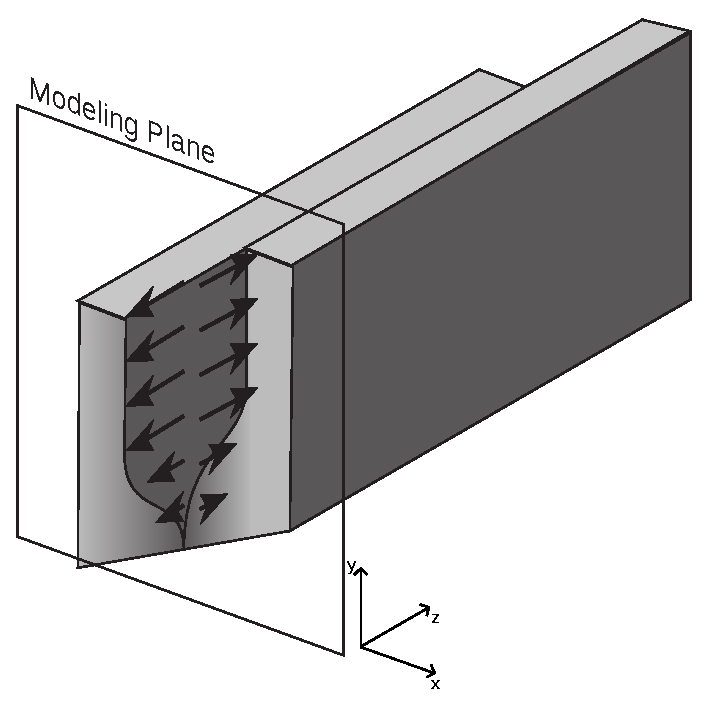
\includegraphics{aps}
\caption{Figure 1\-: Schematic representation of a fault and the modeled plane}
\end{DoxyImage}
 In this case, we can considered that displacement only occurs in the $z$ direction $(v_{x}=v_{y}=0)$. Moreover, under this approximation no magnitude can vary along the $z$ direction $(\frac{\partial}{\partial z}=0)$. Therefore, under this approximation $\varepsilon_{xx}=\varepsilon_{yy}=\varepsilon_{zz}=\varepsilon_{xy}=\varepsilon_{yx}=0$ and $\omega_{xx}=\omega_{yy}=\omega_{zz}=\omega_{xy}=\omega_{yx}=0$ and the governing equations are reduced to\-: \[-\partial_x P = f^e_x \] \[-\partial_y P = f^g_y + f^e_y \] \[\partial_x(2\eta_{ef}\varepsilon_{xz})+\partial_y(2\eta_{ef}\varepsilon_{yz})=f^e_z\]

where \[f^e_x = -\partial_x \left\{\eta_{ef}\left[ \frac{1}{\mu\Delta t} \tau^{t-1}_{xx} + \frac{1}{\mu} \left(\omega^{t-1}_{xz}\tau^{t-1}_{zx} - \tau^{t-1}_{xz}\omega^{t-1}_{zx} \right) \right] \right\} -\partial_y \left\{\eta_{ef}\left[ \frac{1}{\mu\Delta t} \tau^{t-1}_{yx} + \frac{1}{\mu} \left(\omega^{t-1}_{yz}\tau^{t-1}_{zx} - \tau^{t-1}_{yz}\omega^{t-1}_{zx} \right) \right] \right\} \]

\[f^e_y = -\partial_x \left\{\eta_{ef}\left[ \frac{1}{\mu\Delta t} \tau^{t-1}_{xy} + \frac{1}{\mu} \left(\omega^{t-1}_{xz}\tau^{t-1}_{zy} - \tau^{t-1}_{xz}\omega^{t-1}_{zy} \right) \right] \right\} -\partial_y \left\{\eta_{ef}\left[ \frac{1}{\mu\Delta t} \tau^{t-1}_{yy} + \frac{1}{\mu} \left(\omega^{t-1}_{yz}\tau^{t-1}_{zy} - \tau^{t-1}_{yz}\omega^{t-1}_{zy} \right) \right] \right\} \]

\[f^e_z = -\partial_x \left\{\eta_{ef}\left[ \frac{1}{\mu\Delta t} \tau^{t-1}_{xz} + \frac{1}{\mu} \left(\omega^{t-1}_{xz}\tau^{t-1}_{zz} - \tau^{t-1}_{xx}\omega^{t-1}_{xz} - \tau^{t-1}_{xy}\omega^{t-1}_{yz} \right) \right] \right\} -\partial_y \left\{\eta_{ef}\left[ \frac{1}{\mu\Delta t} \tau^{t-1}_{yz} + \frac{1}{\mu} \left(\omega^{t-1}_{yz}\tau^{t-1}_{zz} - \tau^{t-1}_{yx}\omega^{t-1}_{xz} - \tau^{t-1}_{yy}\omega^{t-1}_{yz} \right) \right] \right\}\]

The velocity at time $t$ only appears in the $z$ component equation. Therefore, we will only solve said equation. In terms of $v_z$ the equation is\-: \[\partial_x \left(\eta_{ef}\partial_x v_z \right) + \partial_y \left(\eta_{ef}\partial_y v_z \right) = f^e_z \]

and for uniform effective viscosity we obtain the Poisson equation\-:

\[\eta_{ef}\Delta v_z = f^e_z \]\hypertarget{index_model}{}\section{Modeling}\label{index_model}
\hypertarget{index_setup}{}\subsection{Setup}\label{index_setup}
Here we will solve the visco-\/elastic equation in a two-\/dimensional domain of dimensions $a$ by $b$. We will solve for the velocity in the direction perpendicular to the plane $(v_z)$ caused by a fault also perpendicular to the modeled plane.

There are four possible boundary conditions\-:


\begin{DoxyItemize}
\item $\Gamma_0$ -\/ The locked part above the fault, with imposed zero velocity, $v_z=0$ (homogeneous Dirichlet boundary conditions).
\item $\Gamma_1$ -\/ Regions of imposed velocity, $v_z=V$ (non-\/homogeneous Dirichlet boundary conditions).
\item $\Gamma_2$ -\/ Zero tangential stress boundaries, $\boldsymbol{n} \cdot \tau - P =0$ (homogeneous Neumann boundary conditions).
\item $\Gamma_3$ -\/ Imposed tangential stress $\boldsymbol{n} \cdot \tau - P =S$ (non-\/homogeneous Neumann boundary conditions).
\end{DoxyItemize}\hypertarget{index_weak_form}{}\subsection{The Weak Form}\label{index_weak_form}
In order to solve the equation using the Finite Element Method we need to derive the weak form. We will begin with the partial differential equation that governs the velocity in a visco-\/elastic medium under the anti-\/plane shear approximation\-: \[ \nabla \left(\eta_{ef}\nabla v_z\right)=f^e_z\]

where i=1,2. First we multiply the equation from the left by a test function $v$, and then we integrate over the whole domain\-: \[\int_{\Omega} v \cdot \nabla\left(\eta_{ef}\nabla v_z \right) = \int_{\Omega} v \cdot f^e_z \phi \]

Integrating by parts and using the Gauss theorem \[ \int_{\Omega} \nabla v \cdot \eta_{ef}\nabla v_z = -\int_{\Omega} v \cdot f^e_z + \int_{\partial \Omega} v \cdot \eta_{ef} \boldsymbol{n} \nabla v_z \]

We can integrate by parts the term corresponding to the internal elastic force if we take into account that it is in fact the divergence of another function $ f^e_z = -\partial_i g^e_{iz} $. Therefore, we obtain\-: \[ \int_{\Omega} \nabla v \cdot \eta_{ef}\nabla v_z = -\int_{\Omega} \nabla v \cdot \boldsymbol{g^e_z} + \int_{\partial \Omega} v \cdot \eta_{ef} \boldsymbol{n} \nabla v_z + \int_{\partial \Omega} v \cdot \boldsymbol{n} \boldsymbol{g^e_z} \]

Considering that the boundary terms are related to the stress tensor $ \tau_{ij}$ we obtain\-: \[ \int_{\Omega} \nabla v \cdot \eta_{ef}\nabla v_z = -\int_{\Omega} \nabla v \cdot \boldsymbol{g^e_z} + \int_{\partial \Omega} v \cdot \boldsymbol{n} \tau_{iz} \]

or\-: \[ \left( \nabla v, \eta_{ef}\nabla v_z \right)_{\Omega} = - \left( \nabla v, \boldsymbol{g^e_z} \right)_{\Omega} + \left(v, \boldsymbol{n} \boldsymbol{\tau_{z}} \right)_{\partial \Omega} \]

where $\boldsymbol{\tau_{z}} = \tau_{iz}$.

In those boundaries where the velocity is imposed (Dirichlet boundary conditions), this is $\Gamma_0$ and $\Gamma_1$,the test function $v = 0$. The contribution of those boundaries in which the imposed tangential stress is zero (i.\-e., $\Gamma_2$) will not contribute to the right hand side either. On the other hand,those boundaries in which we impose a non-\/zero tangential stress (non-\/homogeneous Neumann boundary conditions), this is $\Gamma_3$, the test functions $v \neq 0$, and that part of the boundary integral has to be included in the weak form. \[ \left( \nabla v, \eta_{ef}\nabla v_z \right)_{\Omega} = - \left( \nabla v, \boldsymbol{g^e_z} \right)_{\Omega} + \left(v, S \right)_{\Gamma^3} \]

where the operator $(a, b)$ is $ \int a \cdot b $ and $S$ is the imposed tangential stress at the boundary.

We can now replace the exact solution $ v_z $ for an approximate solution in terms of the shape functions, $ \sum_{j} U_j v_j(\boldsymbol{x}) $. Here $U_j$ are the expansion coefficients we need to determine to find the approximate solution to the laplace equation. Then, the problem is reduced to solving \[AU=B\] where the matrix A and the vector B are defined as\-: \[A_{ij} = (v_i,v_j)_{\Omega}\] \[B_i = -(\nabla v_i, \boldsymbol{g^e_z})_\Omega + (v_i, S)_{\Gamma_3} \]\hypertarget{index_adaptive_refinement}{}\subsection{Adaptive Mesh Refinement in Time Dependent Problems}\label{index_adaptive_refinement}
Every time step we need to use the solution from the two last time steps and the visco-\/elastic stress from the previous one. The old solutions are stored in a \href{https://www.dealii.org/8.4.0/doxygen/deal.II/classVector.html}{\tt Vector} with as many elements as the degrees of freedom the problem has. The old stress is stored at each quadrature and can be accessed through a user pointer that each cell holds. Every time the mesh is refined, the number of cells and degrees of freedom changes, therefore, as part of the mesh refinement we need to transfer the solution vectors and the old stress from the old mesh to the new one. For the solution vectors we just need to use \href{https://www.dealii.org/8.4.0/doxygen/deal.II/classSolutionTransfer.html}{\tt Solution\-Transfer} (see for example \href{https://www.dealii.org/8.2.0/doxygen/deal.II/step_26.html#codeHeatEquationrefine_meshcode}{\tt Step-\/26}).

Transferring the old stress is slightly more complicated, we need to transfer the data sotred in the quadrature points to a finite element field that is defined everywhere so that we can later transfer it to the new mesh (using \href{https://www.dealii.org/8.4.0/doxygen/deal.II/classSolutionTransfer.html}{\tt Solution\-Transfer} and then interpolate it to the new quadrature points. We need a discontinuous field that matches the values in the quadrature points (we will use a Discontinuous Galerking finite element \href{https://www.dealii.org/8.2.0/doxygen/deal.II/classFE__DGQ.html}{\tt F\-E\-\_\-\-D\-G\-Q}). 